\chapter{\label{ch:1-intro}Introduction} 

\graphicspath{{figures/ch1/}}

\minitoc

\section{General introduction}

\section{Pancreatic islets and the \textgreek{b}-cell}

Pancreatic islets are endocrine cells which are responsible for maintaining glucose homeostasis.
There are roughly one million islets in a human pancreas, constituting 1-2\% of the total pancreatic mass.
Islets consist of three principal cell types; insulin secreting \textgreek{b}-cells, glucagon secreting \textgreek{a}-cells and somatostatin secreting \textgreek{d}-cells.
Islets respond to increases in blood glucose by releasing insulin, which acts on peripheral tissues to increase glucose uptake and reduce blood glucose levels.
Conversely, decreases in blood glucose leads to the release of glucagon, which acts on those tissues to stimulate glucose production and increase blood glucose.

\section{Architecture of the pancreatic K\ATP{} channel}

ATP-sensitive potassium (K\ATP{}) channels are present in many tissues, where they couple the metabolic state of a cell to its electrical activity by regulating the flow of K\textsuperscript{+} across the membrane.
K\ATP{} channels are an octameric complex, comprised of four inwardly-rectifying potassium channel subunits (Kir6.1 or Kir6.2), each of which is associated with a sulphonylurea receptor subunit (SUR1, SUR2A or SUR2B).
In pancreatic \textgreek{b}-cells, the K\ATP{} channel isoform is composed of Kir6.2 and SUR1.
Together, Kir6.2 and SUR1 form a complex nearly a megadalton in size and over 15 nanometres across (Figure \ref{ch1fig:katp_cartoon}, \ref{ch1fig:sur_topdown}).

Inwardly-rectifying potassium channels are so named because they allow K\textsuperscript{+} to flow more easily into the cell than out of it (Figure \ref{ch1fig:rectification}).
This phenomenon is a consequence of voltage-dependent pore blockade by intracellular divalent cations (especially Mg\textsuperscript{2+}) and polyamines.
At depolarising membrane potentials, blockers are driven into the pore and K\textsuperscript{+} current is blocked, while at hyperpolarising potentials the blockers and cleared and K\textsuperscript{+} current can flow.
Strongly rectifying Kir channels display drastically reduced conductance at potentials more positive than the K\textsuperscript{+} reversal potential.
In contrast, Kir6.2 is a weak rectifier, and allows substantial current to flow at more positive potentials.

In addition to voltage, Kir6.2 is regulated by two endogenous ligands; 
phosphatidylinositol 4,5-bisphosphate (PIP\textsubscript{2}) and adenine nucleotides (Figure \ref{ch1fig:kir_struct}).
The binding of adenine nucleotides to Kir6.2 leads to closure of the channel pore, while the binding of PIP\textsubscript{2} promotes the opening of the pore (Figure \ref{ch1fig:shyng_trace}).
Activation by PIP\textsubscript{2} is a mechanism common to the whole Kir family, wherease inhibition by nucleotides is unique to the Kir6 subfamily.

\begin{figure}[h]
	\centering
	\begin{subfigure}[t]{0.5\textwidth}
		\caption{}\label{ch1fig:rectification}
		\centering
		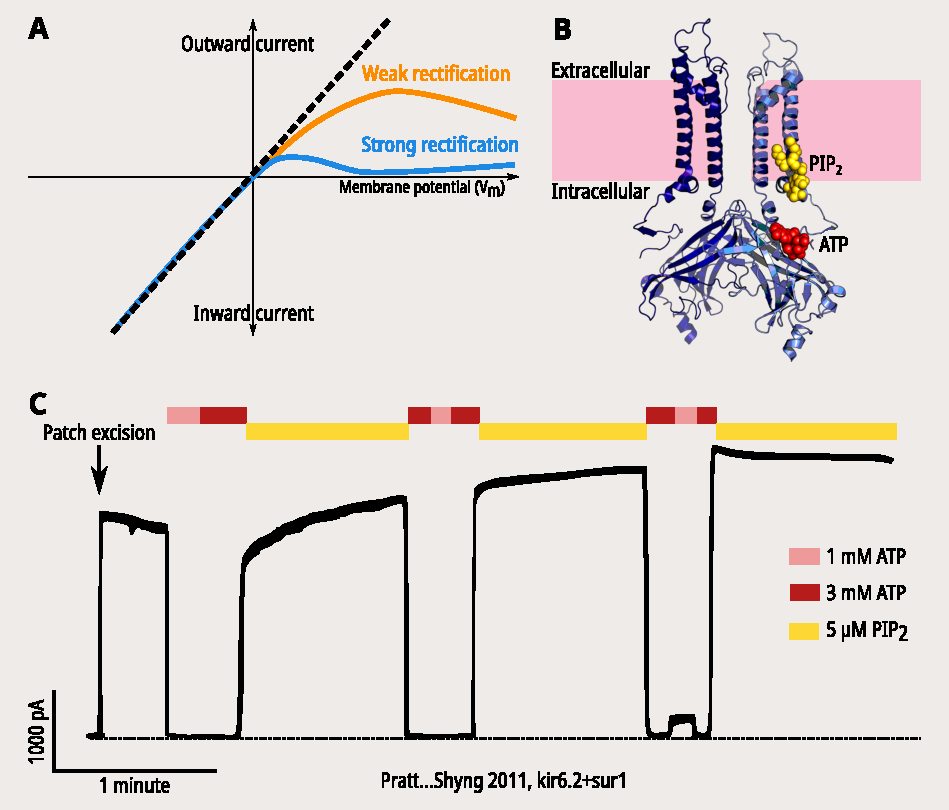
\includegraphics[width=\textwidth]{rectification.pdf}
	\end{subfigure}
	\hfill
	\begin{subfigure}[t]{0.4\textwidth}
		\caption{}\label{ch1fig:kir_struct}
		\centering
		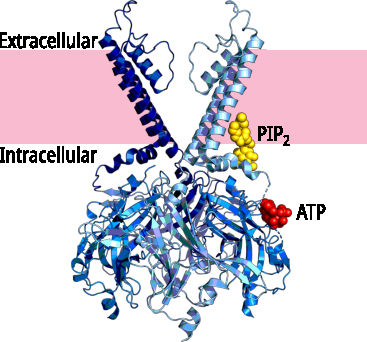
\includegraphics[width=\textwidth]{kir_structure.pdf}
	\end{subfigure}
	\vfill
	\begin{subfigure}[t]{0.9\textwidth}
		\caption{}\label{ch1fig:shyng_trace}
		\centering
		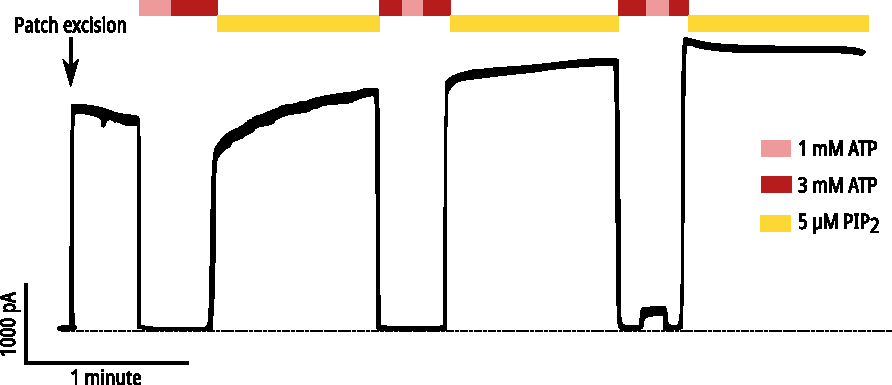
\includegraphics[width=\textwidth]{shyng_atp_pip_trace.pdf}
	\end{subfigure}
	\caption[Structure of Kir6.2]{
		\subref{ch1fig:rectification} Current-voltage plot demonstrating inward rectification of Kir channels.
		Here, the reversal potential of potassium (\textit{E\textsubscript{K}}) is set to zero, i.e. there is an equal concentration of K\textsuperscript{+} on each side of the membrane.
		Weak rectifiers such as Kir6.2 exhibit only a weak voltage dependent decline in conductance (visualised as a departure from the dashed line of an ideal conductor).
		(Kind of adapted from Handbook of Ion Channels).
		\subref{ch1fig:kir_struct} Cryo-EM structure of Kir6.2 (PDB \#6BAA) captured with ATP bound (red) and with the proposed binding position of PIP\textsubscript{2} visualised by alignment of the channel with the X-ray structure of Kir2.2 solved in compex with a short-chain dioctanoyl (diC8) PIP\textsubscript{2} (PDB \#6C3I).
		The plasma membrane is shown in pink.
		(Kind of adapted from Mike's JGP review).
		\subref{ch1fig:shyng_trace} Macroscopic currents from Kir6.2 channels coexpressed with SUR1 in excised patches from cultured cells, adapted from (Pratt/Shyng, 2011).
		Perfusion of ATP or PIP\textsubscript{2} is indicated by coloured bars, and demonstrates the contrasting effects of these two ligands on channel activity.
	}
	\label{ch1fig:kir_breakdown}
\end{figure}

SUR1 is a member of the ATP-binding cassette (ABC) family of transporters.
While other ABC proteins transport substrate across the membrane, SUR1 does not appear to do so; instead it acts to modulate the function of its associated ion channel.
The cystic fibrosis transmembrane conductance regulator (CFTR) is another member of the ABC family, and is an ion channel in its own right, capable of conducting chloride across the membrane.
Like other ABC proteins, SUR1 contains two sets of transmembrane domains (TMD1 and TMD2) and two cytosolic nucleotide binding domains (NBD1 and NBD2).
Unique to SUR is the presence of an additional transmembrane domain (TMD0) N-terminal to the core of the protein, and this domain forms the primary contact between SUR1 and Kir6.2.

The NBDs of ABC transporters are highly conserved, and consist of two subdomains: a larger RecA-like subdomain found in other P-loop ATPases, and a smaller \textgreek{a}-helical subdomain which is unique to ABC transporters.
There are three key structural motifs present in these subdomains: the RecA-like subdomain contains the Walker A (W\textsubscript{A}) and B (W\textsubscript{B}) motifs, while the \textgreek{a}-helical subdomain contains the ABC signature motif (typically LSGGQ).

The two domains come together to form an antiparallel dimer with two nucleotide binding sites (NBS1 and NBS2) at the interface, such that NBS1 is formed from the W\textsubscript{A} and W\textsubscript{B} motifs of NBD1 and the signature motif from NBD2, whereas NBS2 is formed from the W\textsubscript{A} and W\textsubscript{B} motifs of NBD2 and the signature motif from NBD1.
NBS2, also known as the consensus site as it is more similar in sequence to other ABC family members, is catalytically competent and able to hydrolyse ATP.
In contrast, NBS1 is the degenerate site, with a less conserved sequence and an inability to catalyse hydrolysis of ATP.

\begin{figure}[h]
	\centering
	\begin{subfigure}[t]{0.4\textwidth}
		\caption{}\label{ch1fig:sur_struct}
		\centering
		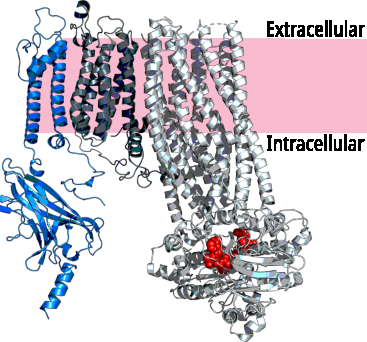
\includegraphics[width=\textwidth]{sur_structure.pdf}
	\end{subfigure}
	\hfill
	\begin{subfigure}[t]{0.5\textwidth}
		\caption{}\label{ch1fig:nbd_struct}
		\centering
		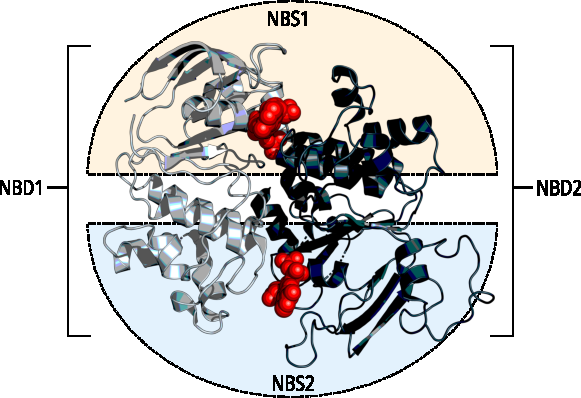
\includegraphics[width=\textwidth]{nbd_structure.pdf}
	\end{subfigure}
	\caption[Structure of SUR1]{
		\subref{ch1fig:sur_struct} Cryo-EM structure of SUR1 captured with a nucleotide (shown in red) bound at each NBS (PDB \#6C3P).
		A single SUR1 subunit is shown, with TMD1 and TMD2 in white and TMD0 in grey.
		A single Kir6.2 subunit is also shown in blue to show the interface between subunits.
		The plasma membrane is displayed in pink.
		\subref{ch1fig:nbd_struct} Top-down view of the NBDs from the same cryo-EM structure.
		NBD1 is on the left in white, NBD2 is on the right in grey, and the two NBSs are higlighted; NBS1 in orange and NBS2 in blue.
		Adapted from Mikes JGP review.
	}
\end{figure}

\section{Ligand-independent regulation of the pancreatic K\ATP{} channel}

\subsection{Assembly and trafficking}

Biogenesis of K\ATP{} channels occurs in the endoplasmic reticulum (ER), and is an important checkpoint in determining surface expression and channel stoichiometry \cite{zerangue_new_1999-1, martin_pharmacological_2013}.
The precise nature of the events which occur between subunit translation and insertion of octameric K\ATP{} into the cell membrane are not fully mapped out, but studies have highlighted some important quality control steps in this process which regulate K\ATP{} channel expression.
When Kir6.2 or SUR1 are expressed alone in heterologous systems, they are retained in the ER \cite{zerangue_new_1999-1}.
This mechanism is achieved through the exposure of a three amino acid ER-retention motif (RKR) in the cytoplasmic domains of both Kir6.2 and SUR1.
Only upon complete assembly of the channel complex are the RKR motifs masked, allowing forward trafficking of K\ATP{} to the cell surface.
Deletion of the RKR motif \cite{tucker_truncation_1997}, or mutation of the motif to AAA \cite{zerangue_new_1999-1}, results in unregulated surface expression of individual subunits and/or partially assembled channel complexes.
Addition of a GFP label to the C-terminus of Kir6.2 is also sufficient to allow trafficking of subunits to the cell surface in the absence of SUR1 \cite{john_sulphonylurea_1998-1}.

In addition to the RKR motif, there are two N-linked glycosylation sites on SUR1 (N10 and N1050) which are required for cell surface expression \cite{conti_membrane_2002}.
Mutation of these sites to glutamines results in retention in the ER and drastically reduced expression of K\ATP{} on the cell surface.
This mechanism is thought to be separate to that for the ER-retention motif, as mutation of RKR to AAA is not sufficient to drive surface expression of the glycosylation mutants \cite{conti_membrane_2002}.

A putatitive third site of trafficking regulation is in the C-terminus of SUR1.
Mutation or deletion of a dileucine motif 16 amino acids distal to the C-terminal of SUR1 results in reduced surface expression of K\ATP{} channels in COSm6 cells \cite{sharma_c_1999}.
This reduction in expression is not rescued by C-terminal truncation of Kir6.2, indicating that this result is not due to masking of the RKR retention motif.
The dileucines are therefore suggested to promote forward trafficking of assembled channel complexes to the cell membrane \cite{sharma_c_1999}.
Expression of K\ATP{} channels expressed in \textit{Xenopus} oocytes is also dramatically reduced by truncation of the C-terminal 42 amino acids of SUR1 \cite{vedovato_role_2018}.
However, longer deletions of the SUR1 C-terminus did not reduce surface expression of channels in HEK293 cells \cite{giblin_cytoplasmic_2002}, and other modifications of the SUR1 C-terminus do not exhibit effects on surface expression \cite{schwappach_molecular_2000}.
The precise role of the dileucine motif remains unclear, and is potentially confounded by the use of expression system \cite{giblin_cytoplasmic_2002, martin_pharmacological_2013}

Failure of the channel complex to pass these three checkpoints results in ER-associated degradation (ERAD), a common pathway shared by most membrane and secretory proteins \cite{bonifacino_ubiquitin_1998, yan_role_2005}.
Both SUR1 and Kir6.2 are substrates for polyubiquitination, both when heterologously expressed and in INS-1 cells \cite{yan_role_2005}.
Application of proteasome inhibitors both reduces the rate of degradation for Kir6.2 and SUR1, and increases the surface expression of K\ATP{} channels by increasing their biogenesis efficiency \cite{yan_role_2005}.

The surface expression of K\ATP{} channels is therefore controlled by a variety of different quality control mechanism to ensure that only correctly assembled octameric channel complex reach the cell membrane.
Mutations which lead to defects in assembly and trafficking are therefore a common cause of congential hyperinsulinemia (HI).
These mutations are found throughout both Kir6.2 and SUR1, although they are more commonly found in SUR1 \cite{martin_pharmacological_2013}.

Interestingly, sulphonylureas are able to act as pharmacological chaperones and rescue surface expression of several mutations which would otherwise not traffic to the cell surface \cite{yan_sulfonylureas_2004, yan_sulfonylureas_2006, yan_congenital_2007, yan_congenital_2007-2, martin_pharmacological_2016}.
Sulphonylureas bind directly to the channel during biogenesis, as mutation of residues in SUR1 which are critical for sulphonylurea binding abolished or reduced the effectiveness of expression rescue \cite{yan_sulfonylureas_2006}.
Pharmacological chaperoning requires full assembly of the channel complex, as the presence of Kir6.2 was required to rescue expression of trafficking mutants even when the SUR1 RKR motif was mutated to AAA \cite{yan_sulfonylureas_2006}.
In addition, reducing the temperature at which cells are cultured can rescue some trafficking defects \cite{yang_low_2005}.

\begin{figure}[h]
	\centering
	\begin{subfigure}[t]{0.9\textwidth}
		\caption{}\label{ch1fig:katp_cartoon}
		\centering
		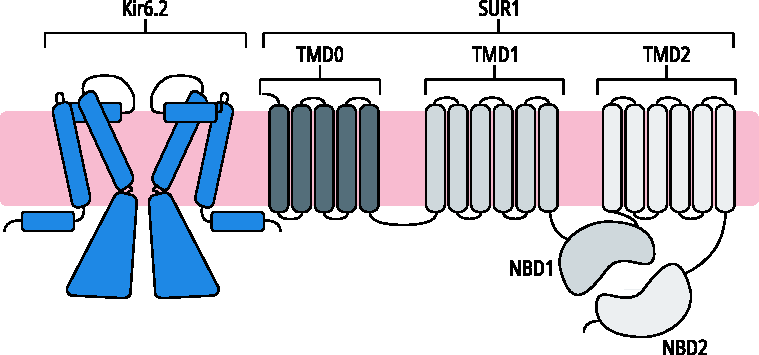
\includegraphics[width=\textwidth]{katp_cartoon.pdf}
	\end{subfigure}
	\vfill
	\begin{subfigure}[t]{0.45\textwidth}
		\caption{}\label{ch1fig:sur_topdown}
		\centering
		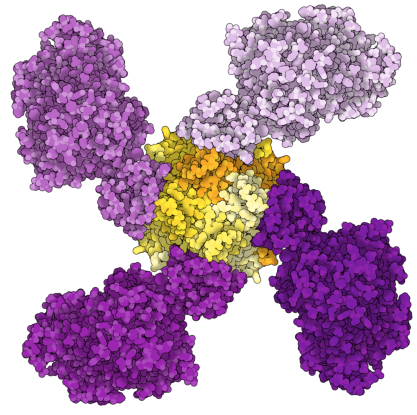
\includegraphics[width=\textwidth]{sur_topdown_propellor.pdf}
	\end{subfigure}
	\hfill
	\begin{subfigure}[t]{0.45\textwidth}
		\caption{}\label{ch1fig:sur_ctd}
		\centering
		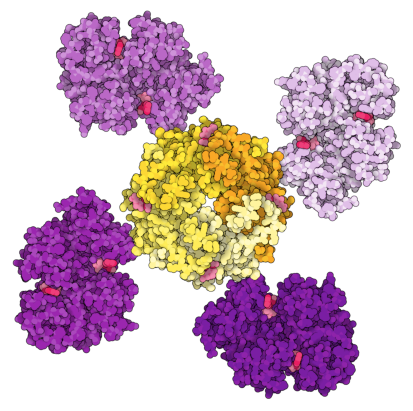
\includegraphics[width=\textwidth]{sur_topdown_ctd_propellor.pdf}
	\end{subfigure}
	\caption[K\ATP{} architecture and nucleotide regulation]{
		\subref{ch1fig:katp_cartoon} Membrane topology of the K\ATP{} channel shown with two Kir6.2 subunits and one SUR1 subunit.
		\subref{ch1fig:sur_topdown} Top-down view of a cryo-EM structure of the K\ATP{} channel (PDB \# 6C3P) solved with nucleotides bound at each of the three canonical binding sites.
		Each SUR1 subunit is shown in a shade of purple, and each Kir6.2 subunit is shown in a shade of orange.
		\subref{ch1fig:sur_ctd} The same view of the structure shown to the left, but with the transmembrane domains removed to reveal the cytoplasmic domains of each subunit only.
		The nucleotides bound to the channel are shown in red.
	}
\end{figure}

\subsection{Regulation of intrinsic gating}

In the absence of nucleotides, K\ATP{} channels are spontaneously active.
Single K\ATP{} channels exhibit bursts of brief openings, separated by long interburst closures \cite{alekseev_ligand-insensitive_1998, babenko_two_1999, li_open_2002, proks_modeling_2009}.
The intrinsic gating of K\ATP{} can therefore be seperated into two separate 'gating' processes; fast (responsible for intraburst closures) and slow (responsible for interburst closures).
While it is helpful to distinguish between fast and slow gating processes to characterise channel kinetics and regulation, doing so does not require the existence of seperate structural gates.
When discussing channel gating 

Fast gating is a property intrinsic to Kir6.2, and the intraburst mean closed time is unaffected by the presence of SUR1 \cite{fang_n-terminal_2006}.
In addition, the presence of nucleotides \cite{alekseev_ligand-insensitive_1998, li_open_2002}, or the presence of PIP\textsubscript{2}

\begin{figure}[h]
	\centering
	\begin{subfigure}[t]{0.45\textwidth}
		\caption{}\label{ch1fig:singles_sur}
		\centering
		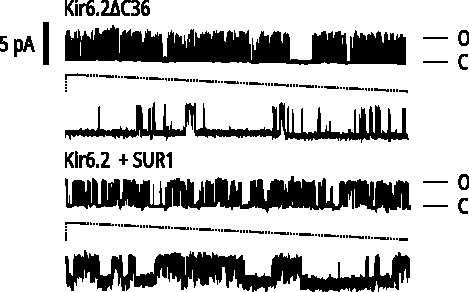
\includegraphics[width=\textwidth]{single_traces_sur.pdf}
	\end{subfigure}
	\hfill
	\begin{subfigure}[t]{0.45\textwidth}
		\caption{}\label{ch1fig:singles_tmd0}
		\centering
		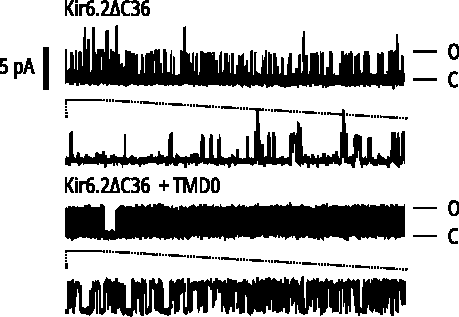
\includegraphics[width=\textwidth]{single_traces_tmd0.pdf}
	\end{subfigure}
	\vfill
	\begin{subfigure}[t]{0.45\textwidth}
		\caption{}\label{ch1fig:sur_shift}
		\centering
		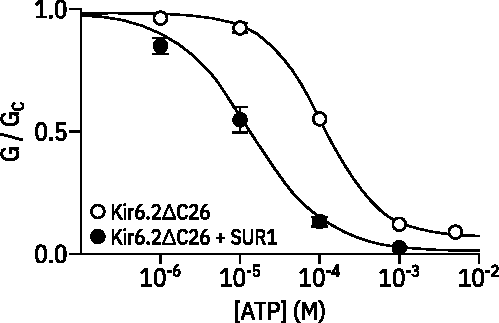
\includegraphics[width=\textwidth]{tucker_sur_shift.pdf}
	\end{subfigure}
	\caption[SUR1 intrinscally modulates Kir6.2]{
		\subref{ch1fig:singles_sur} Single channel recordings of excised patches from cultured cells either expressing Kir6.2 alone with the C-terminal 36 amino acids truncated (Kir6.2\textgreek{D}C36) or coexpressing wild-type Kir6.2 with SUR1.
		Adapted from (Enkvetchakul/Nichols, 2000).
		\subref{ch1fig:singles_tmd0} Single channel recordings of excised patches from cultured cells either expressing Kir6.2\textgreek{D}C36 alone or coexpressing Kir6.2\textgreek{D}C36 with the TMD0 region of SUR1.
		Adapted from (Pratt/Shyng, 2011).
		In both panels, currents were recorded in symmetrical 140 mM K\textsuperscript{+} at a membrane potential of -50 mV and openings are displayed as upward deflections.
		Note that the timescales differ slightly between panels as traces are from two separate papers.
		\subref{ch1fig:sur_shift} Concentration-response relationship of ATP from macroscopic currents excised from \textit{Xenopus} oocytes injected with either Kir6.2\textgreek{D}C26 mRNA alone (open circles), or a mixture of Kir6.2\textgreek{D}C26 and SUR1 mRNAs (closed circles).
		Response is given as the fraction of the slope conductance (G) remaining during exposure to ATP.
		Adapted from (Tucker/Ashcroft, 1997).
	}
\end{figure}

\section{Ligand dependent regulation of the pancreatic K\ATP{} channel}

\begin{figure}[h]
	\centering
	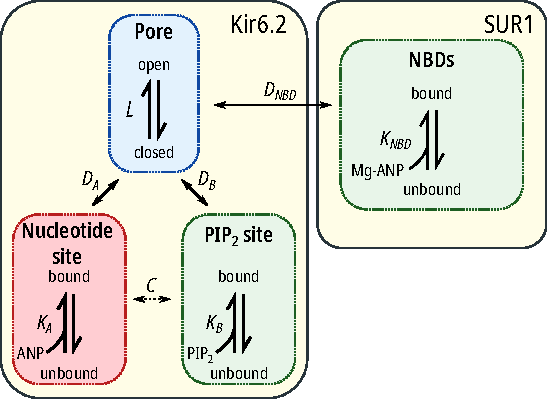
\includegraphics[width=0.7\textwidth]{regulation_diagram.pdf}
	\caption[Modes of regulation of K\ATP{}]{
	Adapted from \cite{puljung_cryo-electron_2018}.
	The open-closed equilibrium of the K\ATP{} channel pore (denoted as $L$) is energetically coupled to three different ligand binding sites.
	The four inhibitory nucleotide binding sites of Kir6.2 (labelled as NBS) bind either ATP or ADP (generalised to ANP) with an equilbrium binding constant $K_A$.
	The four stimulatory PIP\textsubscript{2} binding sites of Kir6.2 bind PIP\textsubscript{2} with an equilbrium binding constant $K_B$.
	The four stimulatory Mg-nucleotide binding site formed by the dimerisation of the NBDs of SUR1 (labelled as NBDs) bind either Mg-ATP or Mg-ADP (generalised to Mg-ANP) with an equilbrium binding constant $K_C$.
	Each binding domain interacts with the channel pore according to the factors $D_A$, $D_B$, and $D_{NBD}$ respectively.
	In addition, there is a potential coupling between the inhibitory nucleotide binding site of Kir6.2 and the stimulatory PIP\textsubscript{2} binding site of Kir6.2 described by the factor $C$.
	}\label{ch1fig:regulation_diagram}
\end{figure}

\subsection{Nucleotide regulation of the pancreatic K\ATP{} channel}

While the binding of adenine nucleotides to the Kir6.2 binding site leads to closure of the pore, binding of nucleotides to either of the two NBSs of SUR1 in the presence of Mg\textsuperscript{2+} activates the channel.
The interplay between the action of nucleotides at these distinct sites (Figure \ref{ch1fig:sur_ctd}) determines the response of the K\ATP{} channel to metabolic changes, and therefore even subtle mutations or modifications to these sites can lead to diseases of insulin secretion.

In addition to its nucleotide binding and sensitivity to sulphonylureas, SUR1 also has intrinsic effects on channel properties.
The presence of SUR1 increases the open probability of the channel pore (Figure \ref{ch1fig:singles_sur}), and this increase is conferred by the TMD0 region (Figure \ref{ch1fig:singles_tmd0}).
Furthermore, coexpression of SUR1 increases the sensitivity of Kir6.2 to inhibition by nucleotides (Figure \ref{ch1fig:sur_shift}).

\subsection{PIP\textsubscript{2} regulation of the pancreatic K\ATP{} channel}

\subsection{Sulphonylurea regulation of the pancreatic K\ATP{} channel}

\section{Fluorescence methods in ion channel research}

\subsection{Fluorescence as a tool}

\subsection{Forster resonance energy transfer}

\subsection{Unnatural amino acid incorporation}

\section{Functional modelling of ion channels}

\subsection{Why?}

\subsection{A model that fits}
